\documentclass[
	a4paper, % Paper size, use either a4paper or letterpaper
	10pt, % Default font size, can also use 11pt or 12pt, although this is not recommended
	unnumberedsections, % Comment to enable section numbering
	twoside, % Two side traditional mode where headers and footers change between odd and even pages, comment this option to make them fixed
]{LTJournalArticle}
\usepackage{amsmath}
\usepackage{multirow}
\addbibresource{refs.bib} % BibLaTeX bibliography file

% A shortened article title to appear in the running head, leave this command empty for no running head

% \footertext{\textit{Journal of Biological Sampling} (2024) 12:533-684} % Text to appear in the footer, leave this command empty for no footer text

\setcounter{page}{1} % The page number of the first page, set this to a higher number if the article is to be part of an issue or larger work

%----------------------------------------------------------------------------------------
%	TITLE SECTION
%----------------------------------------------------------------------------------------

\title{Probabilistic Approaches to 
\\ Energy Conservation in CDNs} % Article title, use manual lines breaks (\\) to beautify the layout

% Authors are listed in a comma-separated list with superscript numbers indicating affiliations
% \thanks{} is used for any text that should be placed in a footnote on the first page, such as the corresponding author's email, journal acceptance dates, a copyright/license notice, keywords, etc
\author{%
	Adarsh Hiremath, Artemas Radik, Andrew Palacci \\
	CS 262: Introduction to Distributed Systems \\
}

\date{May 7, 2023}


%----------------------------------------------------------------------------------------
\newtheorem*{remark}{Remark}
\begin{document}

\maketitle % Output the title section

%----------------------------------------------------------------------------------------
%	ARTICLE CONTENTS
%----------------------------------------------------------------------------------------

\section{1. Introduction}

Throughout the semester, we explored distributed systems fundamentals, implementations, and use cases. One area that especially interested us was replication, since it is so fundamental to the performance and reliability of a variety of distributed systems. In our final project, we wanted to explore an application of replication beyond just fault-tolerance for a client-server chat application.

One such application is content delivery networks (CDNs) --- a type of distributed system that utilizes caching to improve the speed and reliability of content delivery. CDNs strategically place servers in different locations around the world, bringing content closer to users and minimizing the distance between clients and servers.

When a user requests content from a website that uses a CDN, the request is automatically routed to the nearest server in the network, which serves a cached copy of the content. By reducing the distance that data needs to travel over the network, CDNs can help minimize energy consumption and even reduce the carbon footprint of content distribution platforms.

CDNs are widely used by online platforms, serving trillions of requests globally. Therefore, even minor optimizations in CDN modeling can have significant ramifications for energy consumption. In this paper, we identify gaps in the literature regarding the energy efficiency of CDNs and make three significant contributions by doing the following:

\begin{enumerate}
    \item Redefining an existing model and its constraints to be more closely aligned with the energy consumption of modern CDNs.
    \item Providing a strategy along with code to model the optimal number of surrogate servers for a CDN with specific characteristics, identifying the "crossover point" where energy consumption is minimized.
    \item More rigorously examining the choice of cache policies for CDNs, relating them to the various content categories available online today.
\end{enumerate}

Our code can be found \href{https://github.com/andrewp2303/cdnconservation}{\textcolor{blue}{here}}.


\section{2. Existing Approaches}

Several recent papers cover the topic of energy consumption in CDNs. Paper \cite{ulIslam2012} proposes a new energy consumption model for CDN surrogates, compares Uniform and Zipfian redirection policies, and simulates results via a CDNSim testbed \cite{cdnsim}. Critically, the model introduced in \cite{ulIslam2012} does not incorporate network synchronization or transmission costs into its energy model, opting to instead dismiss them. 

Paper \cite{osmanthesis} does account for costs such as that of transmission energy, but also has a general focus on determining optimal CDN cache sizes (both fixed and variable) via a proposed mixed-integer linear programming model. Notably, \cite{osmanthesis} does not have an apparent focus on optimizing CDN surrogate quantities at scale.

Unlike \cite{osmanthesis} and \cite{ulIslam2012}, paper \cite{biancoCDNs2017} assumes that CDN cache sizes are a constant factor of the primary in order to analyze transmission, synchronization, and other costs in-depth. We were able to closely replicate the findings of \cite{biancoCDNs2017}, with small quantitative differences but identical qualitative conclusions. Their model — which is the basis for our proposed model — aligns closely with the reality of the internet. As a result, it's key to understand this paper's approach, which is outlined in the remainder of this section.

\subsection{2.1. Network Topology}

We represent a CDN as a \textit{primary} server, storing the entire data set, connected to several \textit{surrogate} servers, each of which store an equally-sized randomized subset of the primary's contents (note that the randomization is not necessarily uniform). We found this very similar to the primary-backup replication model presented during lecture and in our reading by Budhiraja et al. \cite{BudhirajaNavinPPLB}. The idea is that surrogates sit on the network edge, closer to end users — minimizing cost, latency, and energy usage. 

Both the primary and surrogates sit in the internet, which can be modeled at large as a three-tier network of ISPs (Internet Service Providers). Each tier can be described as follows:
\begin{enumerate}
    \item Tier one ISPs have global reach and are at the top of the hierarchy.
    \item Tier two ISPs are typically regional or country-based, and are responsible for connecting between tier one and tier three ISPs.
    \item Tier three ISPs provide internet connectivity to end users.
\end{enumerate}

\begin{figure}[h]
	\begin{center}
		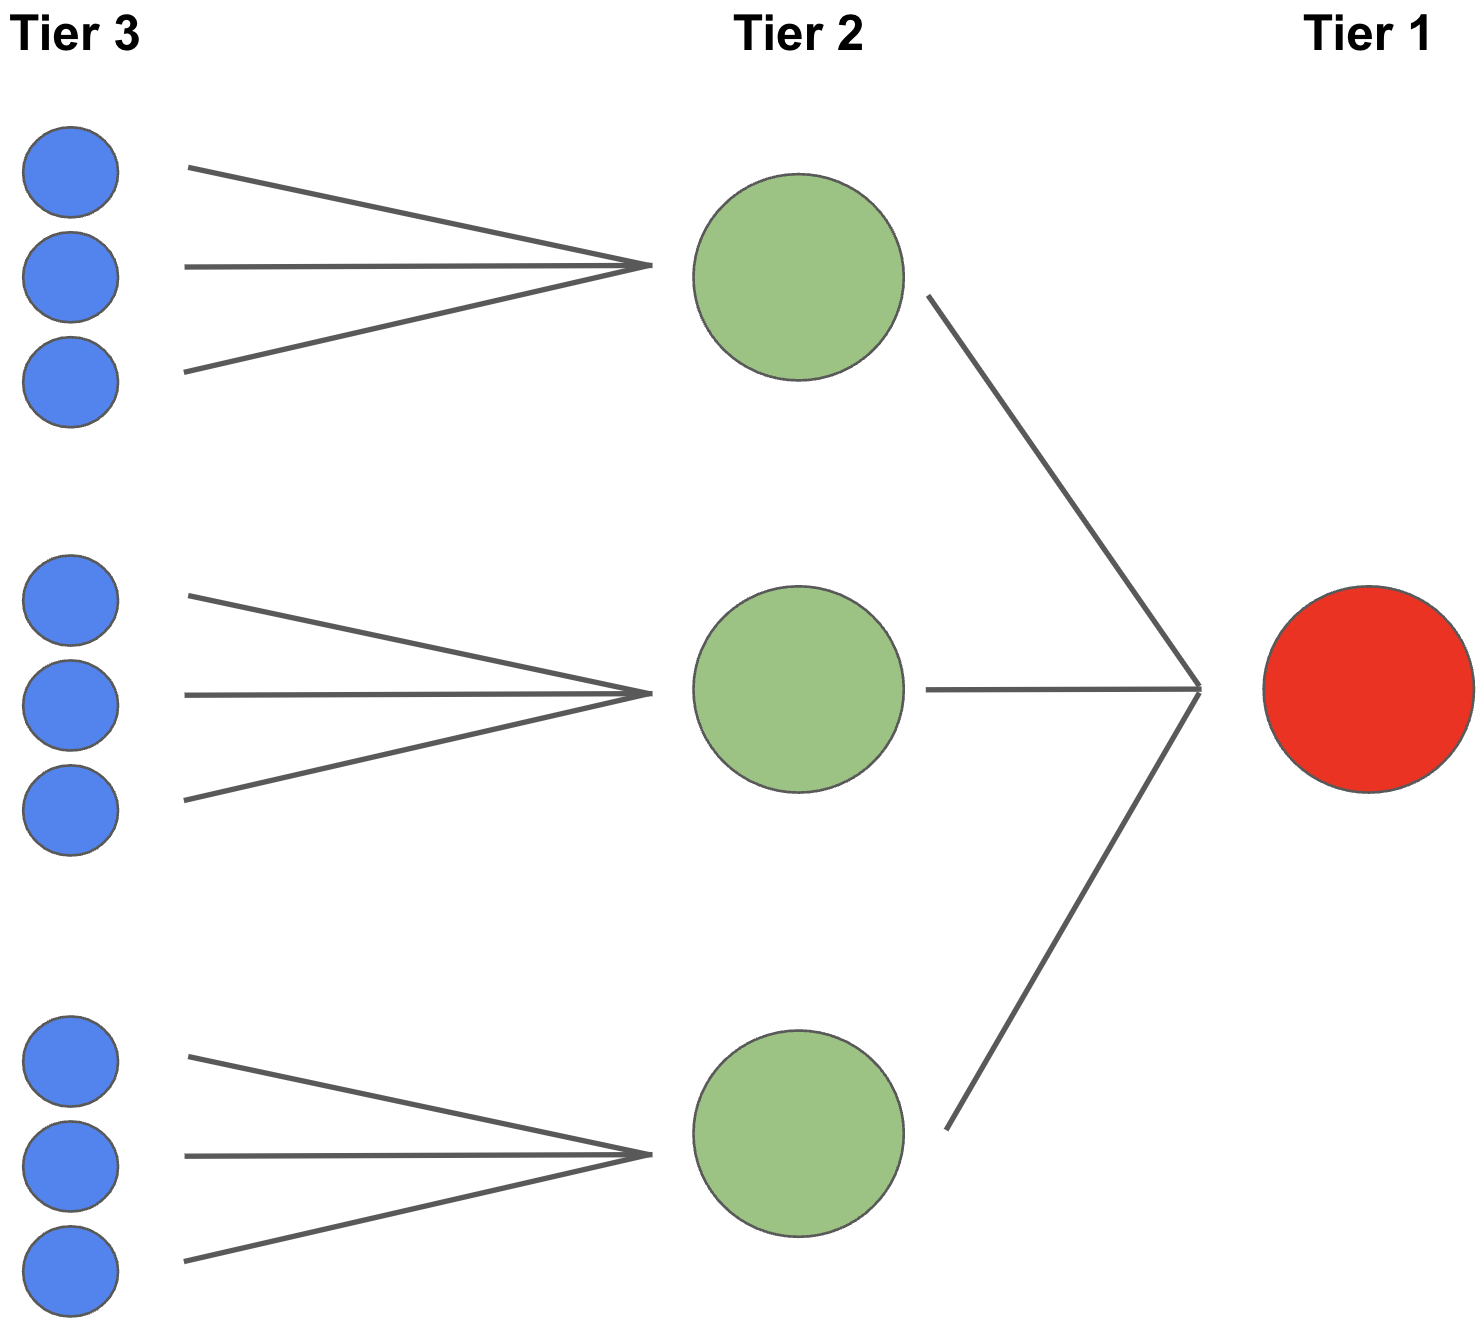
\includegraphics[width=8.1cm]{tier-2.png}
	\end{center}
	\caption{A simplified three-tier ISP topology.}	
\end{figure}

In our model, there are $S$ surrogate servers randomly distributed according to a uniform distribution across all tier three ISPs, with $S < T_2$, the number of tier two ISPs. It is assumed that each tier two ISP is limited to at most one surrogate server in one of its connected tier three ISPs. The graphic below illustrates a tier one ISP as the green bubble, tier two ISPs as orange bubbles, and tier three ISPs as red bubbles. Black squares are surrogate servers, and the primary server is available only via tier one.

\begin{figure}[h]
	\begin{center}
		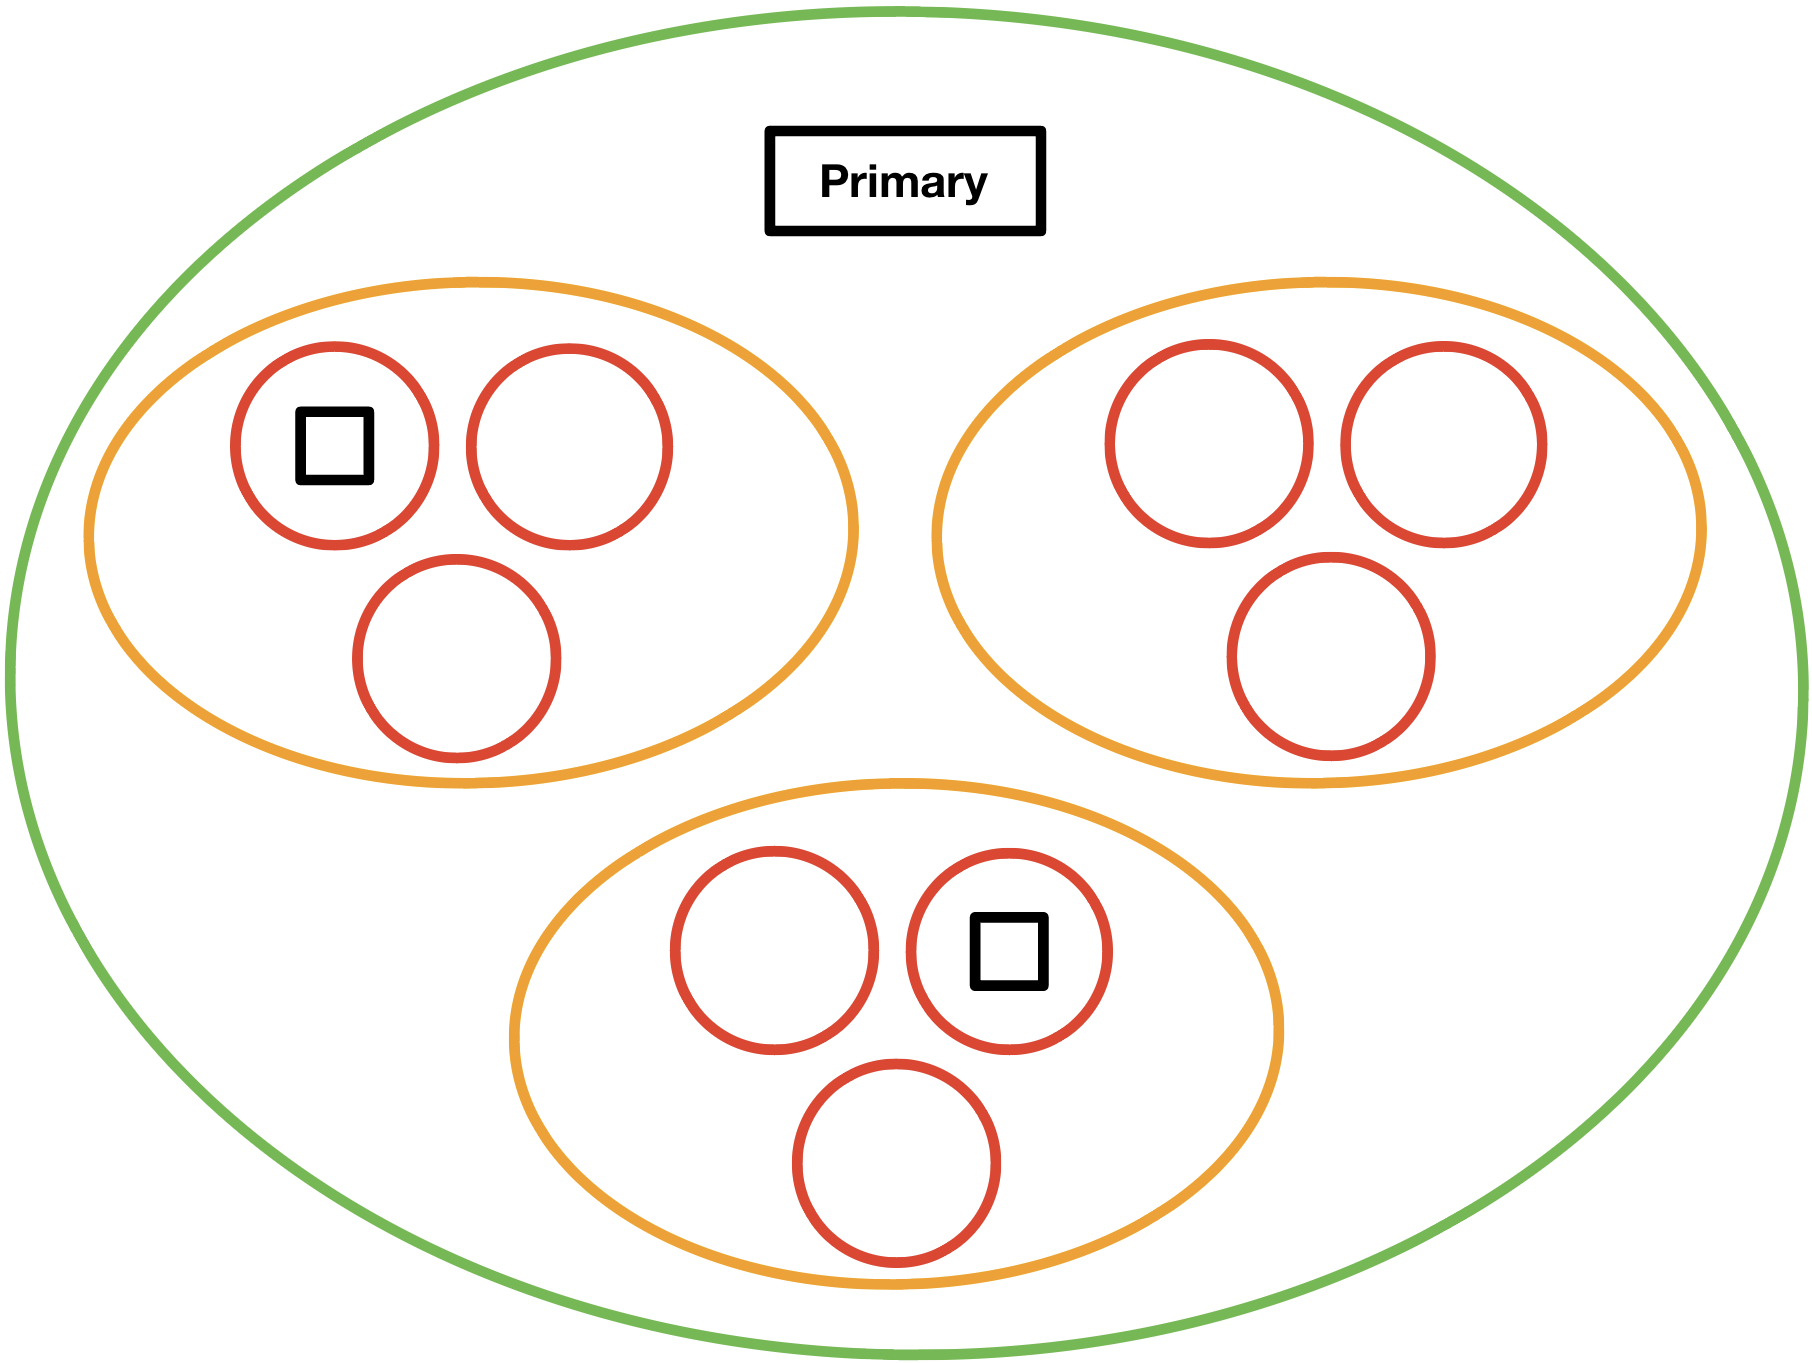
\includegraphics[width=8.1cm]{bubble.jpeg}
	\end{center}
	\caption{Surrogate server constraints visualized in the three-tier ISP topology.}	
\end{figure}
\begin{remark}
The $S < T_2$ constraint is used in the existing literature, though it is rather unintuitive and indeed a limitation of the existing models. Our proposed modifications and calculations, introduced later on, remove the need for this constraint.
\end{remark}



% Efficiently caching content is crucial for highly performant CDNs. Web multimedia data such as text, video, and audio can be exceptionally large, making cache policies essential for ensuring that clients receive data quickly without overburdening the surrogate servers in the CDN. In a simple 3-tier CDN model, we want to move the most popular content to the surrogate servers in the furthest edge of the network - in this case, the 3rd tier.  

% \begin{figure}[h]
% 	\begin{center}
% 		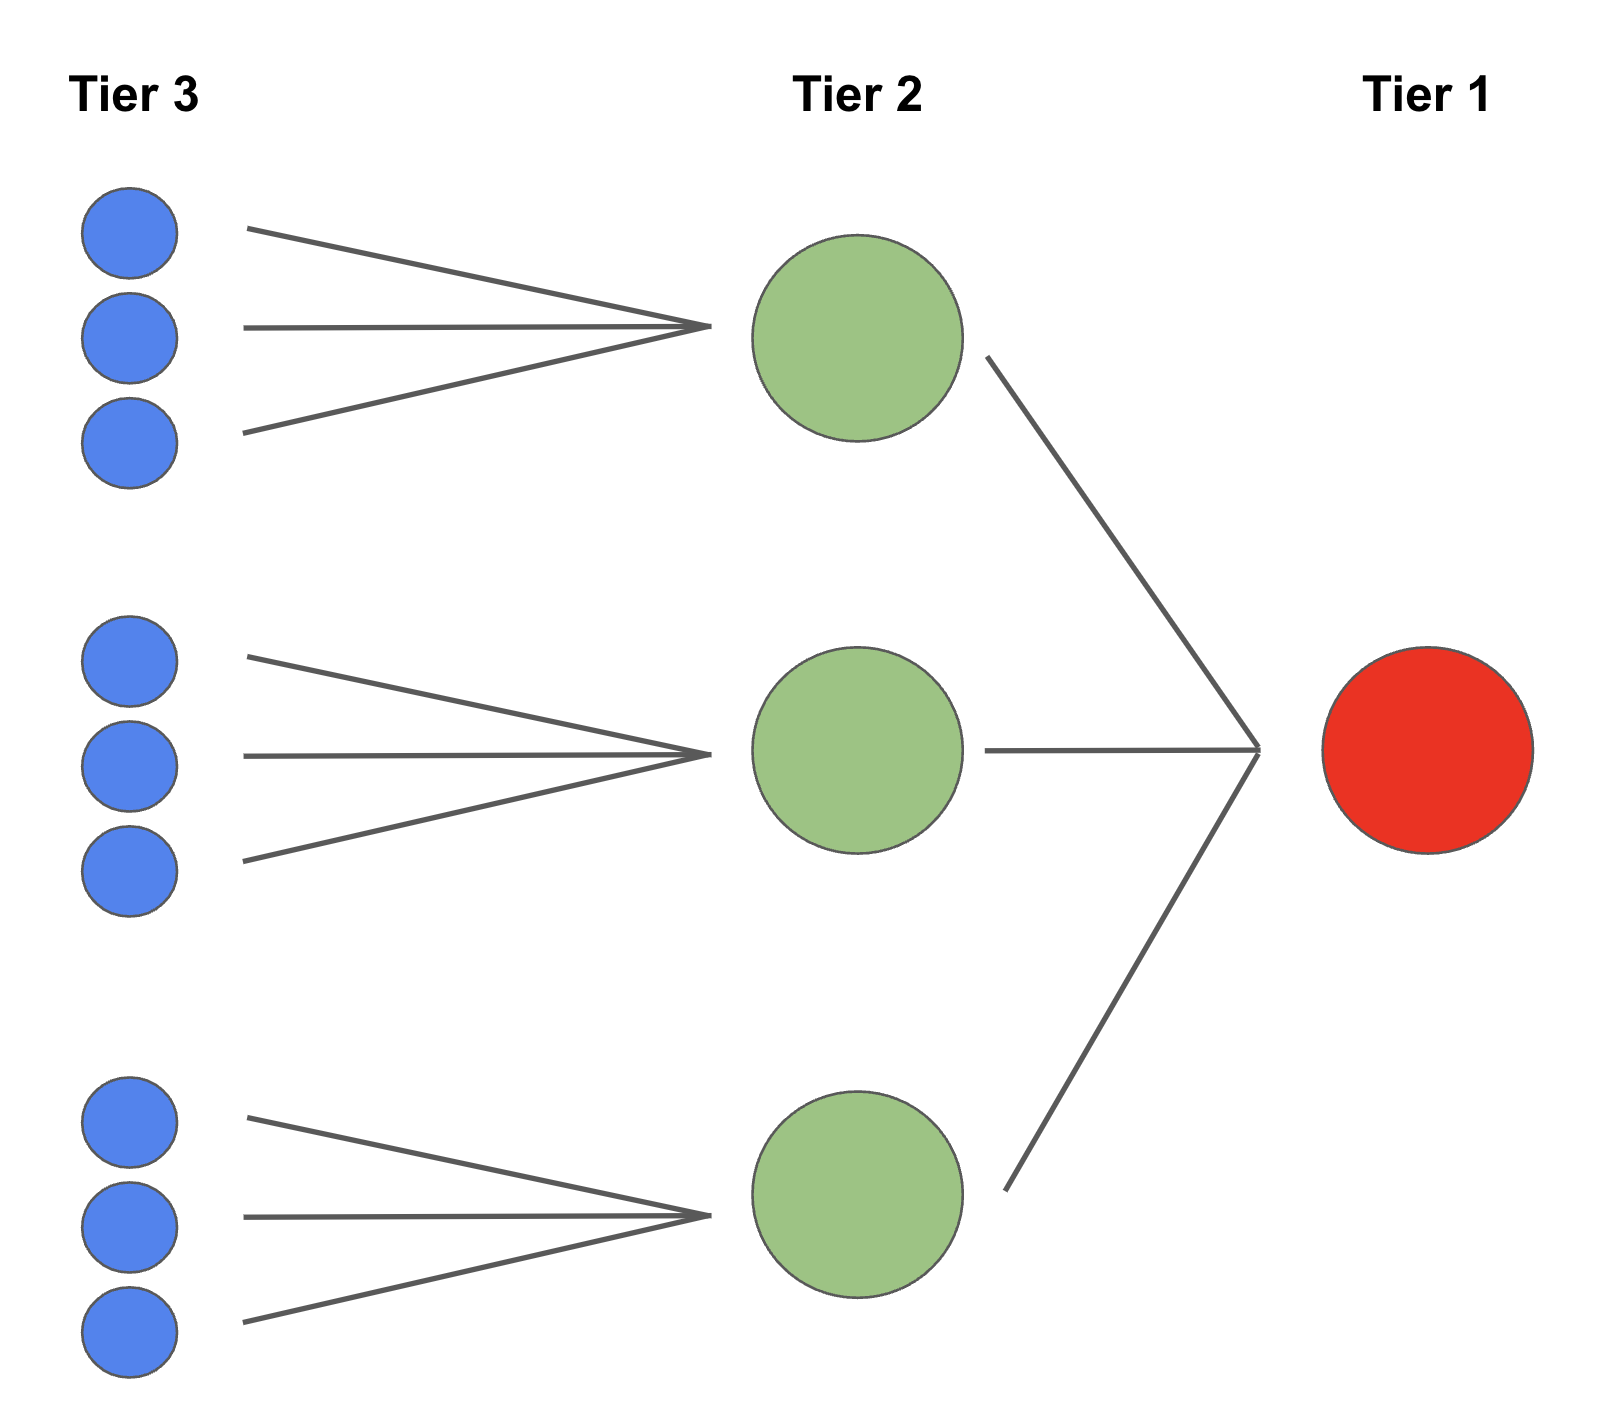
\includegraphics[width=8.1cm]{tier.png}
% 	\end{center}
% 	\caption{A caption for this image.}	
% \end{figure}

% Throughout the paper, we reference the above $3$-tier model. We note the following assumptions and notations about the model: 
% \begin{itemize}
% 	\item Each node in the above model is an ISP. The surrogate servers are placed \textit{within} a tier 3 ISP.
% 	\item The primary server contains all of the content in the CDN, and propagates modified/new content to surrogates according to the cache policy. 
% 	\item There are $T_1$ ISPs in tier $1$, $T_2$ ISPs in tier $2$, and $T_3$ ISPs in tier $3$. 
% 	\item There are $S$ surrogate servers. 
% 	\item $g_3$ represents a group of Tier $3$ ISPs. 
% 	\item The hit probability for each surrogate server is represented as $P_{hit}$.  
	
% \end{itemize}

\subsection{2.2. Cache Policies}
Our model utilizes a cooperative push-based approach, where content is pushed by the primary to each of the surrogates beforehand. The primary keeps a mapping between content and servers, and directs requests accordingly. 

The key problem that cache policies address is how the primary server should allocate content across the available surrogates. Ideally, content is distributed in such a way that maximizes cache hit ratios and (thus) minimizes energy costs.

The first approach requires selecting the data to be stored in each surrogate according to a uniform distribution among the entire data set. In other words, the primary server chooses a random subset of its content to allocate to each surrogate. 

The second approach is popularity-based, and requires as a prerequisite that the primary has an exact ranking of each content's popularity values (these can be view counts, like counts, etc). The data to be stored in each surrogate is randomly selected according to a Zipf distribution with parameter $\alpha = 0.8$. This works because it is shown that many web platforms have content access patterns following an identical distribution \cite{749260}.

\begin{figure}[h]
	\begin{center}
		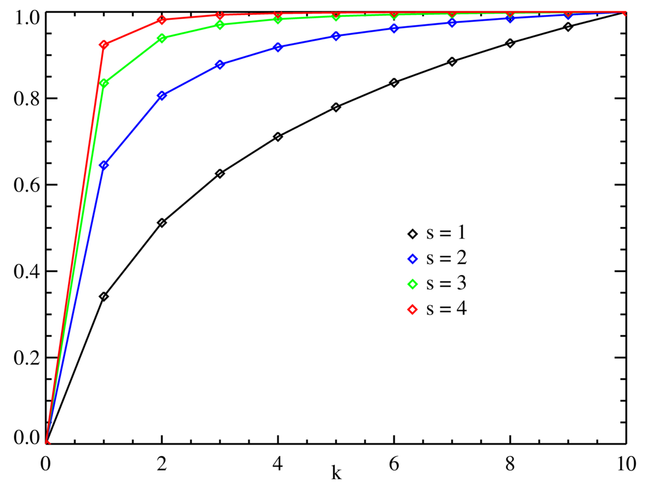
\includegraphics[width=8.1cm]{zipf.png}
	\end{center}
	\caption{A graph of the Zipf distribution CDF with support $k\in\{1, 2, \ldots, 10 \}$ for multiple parameters $s=\alpha \in \{1,2,3,4\}$.}
\end{figure}

\begin{remark}
    Zipf with parameter $\alpha=0.8$ is not always accurate, as later sections will show. This is yet another limitation of the models proposed in existing literature.
\end{remark}

\subsection{2.3  Hit Probability}

The hit probability is the probability that a surrogate server incurs a cache hit. For the uniform approach, the hit probability is trivial: it is simply the size of the surrogate cache as a fraction of the primary storage size. By \cite{749260} and basic probability, the hit probability for the Zipf approach is as follows:

\[ P_{hit}(\alpha, S_C, M) = \sum_{i=1}^{MS_C} \frac{\left( \sum_{k=1}^{M} \frac{1}{k^\alpha}\right)^{-1}}{i^\alpha} = \frac{H_{MS_C, \alpha}}{H_{M,\alpha}} \]

Where $\alpha$ is the Zipf parameter, $M$ is the total number of documents on the primary,  $S_C$ is the surrogate size as a fraction of the primary, and $H_{a,b}$ is the $a$th generalized harmonic number of order $b$. Notably, $P_{hit}(\alpha, S_C, M)$ is equivalent to the CDF of Zipf($\alpha$, $M$) as a function of $MS_C$, as shown above (the final term is the Zipf CDF). Full parameters for our model are outlined below, but note that 
\[P_{hit}(0.8, 0.4, 1000) \approx 0.7847\] 
which we use in our model. This differs from $P_{hit} = 0.82$ as used in \cite{biancoCDNs2017}, which we were unable to replicate, even with their methodology. However, the probabilities are similar enough not to cause any qualitative differences. Interestingly,
\[ \lim_{M\to\infty} P_{hit}(0.8, 0.4, M) \approx 0.8326\]
which suggests that the $P_{hit} = 0.82$ from \cite{biancoCDNs2017} may have been calculated for an arbitrarily larger $M$ than was reported.

\subsection{2.4  Additional Assumptions}
Note the following assumptions that have not yet already been stated:
\begin{enumerate}
    \item Contents are of the same fixed size of $B$ bits.
    \item User requests must originate in tier three ISPs.
    \item Each group of $g_3$ tier three ISPs maps to one tier two ISP, so there are $T_2=\frac{T_3}{g_3}$ tier two ISPs..
    \item User requests are directed to the closest surrogate server containing their requested content, limited to the scope of the originating tier two ISP. If no such surrogate exists, the primary handles the request.
    \item When content is modified the primary instantly propagates it to surrogate servers based on the probability that the surrogate server hosts that content, per the cache policies outlined earlier.
    \item Requests for each content $m$ generate according to a Poisson distribution with parameter $r_m$.
    \item Modifications of each content $m$ generate according to a Poisson distribution with parameter $m_m$.
\end{enumerate}

Note Table 1, which summarizes additional parameters that define our model.
\begin{table}[h]
\scriptsize
\begin{tabular}{ |c|c|c| } 
 \hline
 Symbol & Default Value & Description \\ 
 \hline
 $S$ & variable & number of surrogate servers \\ 
 \hline
 $S_C$ & 40\% & surrogate cache size (relative to primary) \\ 
 \hline
 $M$ & 1000 & total number of contents stored \\ 
 \hline
 $B$ & $10^6$ bits & size of one content \\ 
 \hline
 $t$ & 6000 s & duration of our analysis \\ 
 \hline
 $n_m$ & $S_c \cdot S$ & number of replicas of content $m$ \\ 
 \hline
 $r_m$ & 100, 1000, 10000 & average requests for content $m$ \\ 
 \hline
 $m_m$ & 10, 100 & average modifications for content $m$ \\ 
 \hline
 $H^A_{sd}$ & 3 & hops to fetch content in same Tier 3 ISP \\ 
 \hline
 $H^B_{sd}$ & 14 & hops to fetch content in same Tier 2 ISP \\ 
 \hline
 $H^C_{sd}$ & 25 & hops to fetch content from core network \\ 
 \hline
 $H_{ps}$ & $H^C_{sd}$ & hops from primary to a surrogate \\ 
 \hline
 $T_3$ & 1000 & number of Tier 3 ISPs \\ 
 \hline
 $g_3$ & 20 & number of Tier 3 ISPs per Tier 2 ISP \\ 
 \hline
 $T_2$ & 50 & number of Tier 2 ISPs \\ 
 \hline
 $P_{st}$ & $7.84 \cdot 10^{-12}$ W & storage energy usage per bit \\ 
 \hline
 $E_r$ & $1.2 \cdot 10^{-8}$ J/bit & router energy usage per bit \\ 
 \hline
 $E_l$ & $1.48 \cdot 10^{-9}$ J/bit & link energy usage per bit \\ 
 \hline
 $E_{sr}$ & $2.81 \cdot 10^{-7}$ J/bit & server energy usage per bit \\ 
 \hline
\end{tabular}
\caption{Parameter values for the existing version of our model.}
\end{table}
\normalsize

\subsection{2.5  Energy Consumption Modeling}
Keeping all of these parameters in mind, we establish a cohesive model of the total energy consumed by a CDN in terms of the energy servers use to store data, the energy servers use to perform computations on data and retrieve it for clients, the energy required to keep data on the primary and surrogates synchronized, and finally the energy needed to transmit data to clients. This can be calculated as follows:
\[E_{tot} = E_{storage} + E_{server} + E_{synch} + E_{tx}\]
First, we must consider energy of storing the data across the primary server and all of its surrogates. This involves $n_m$ content replicas of size $B$ bytes each, requiring $P_{st}$ watts over a period of $t$ seconds:
\[E_{storage} = \sum_mBn_mP_{st}t\]
Then, we have $E_{server}$, the energy consumption taken by the computations 
\[E_{server} = \sum_mBr_mP_{sr}\]
Next, we have $E_{synch}$, the energy required to keep all of the surrogate servers up to date with the most recent content. For the purpose of this model, we assume that the primary is aware of which content is cached on each surrogate, and is thus able to efficiently propagate data as mentioned in the aforementioned assumption 5. Here, we incorporate the amount of modifications to content $m$ over the time period $t$, denoted $m_m$. We also touch $H_{ps} + 1$ routers and $H_{ps}$ links for the synchronization of each replica, and thus include these in our energy calculation below:
\[E_{synch} = \sum_mBm_mn_m[E_r(H_{ps} + 1) + E_l(H_{ps})]\]
Finally, in order to calculate our transmission energy, we first need to consider the three distinct cases in which content is transmitted. First is the case $A$ where a client's requested content is found on a surrogate in the same Tier 3 ISP, with probability:
\[P_A = \frac{S}{T_2} \cdot \frac{1}{g_3} \cdot P_{hit}\]
Then, case $B$ entails that case $A$ was not satisfied, but that there is a surrogate in the same Tier 2 ISP that contains the desired content:
\[P_B = \frac{S}{T_2} \cdot \left(1 - \frac{1}{g_3}\right) \cdot P_{hit}\]
Finally, in case $C$, the core network (e.g. the primary server) is the closest server containing the requested content, and thus the data needs to be transmitted from the primary server all the way to the client:
\[P_C = 1 - (P_A + P_B)\]
Given these probabilities, we calculate a combined transmission energy, based on the amount of hops that need to be taken in each of the three cases $A, B, C$, and again the amount of routers and links that need to be touched in the process:
\begin{multline*}
    E_{tx} = P_A\sum_mBr_m[E_r(H^A_{sd} + 1) + E_l(H^A_{sd})] \\
      + P_B\sum_mBr_m[E_r(H^B_{sd} + 1) + E_l(H^B_{sd})] \\
      + P_C\sum_mBr_m[E_r(H^C_{sd} + 1) + E_l(H^C_{sd})] \\
\end{multline*}

\subsection{2.6 Results and Discussion}
Note the results in figures ~\ref{s2uniform0.01} and ~\ref{s2zipf0.01}. In figure \ref{s2uniform0.01}, we see that $E_{tot}$ has a positive slope, implying that scaling the number of surrogates in the CDN indeed increases our energy impact. Such a graph might suggest that a network administrator should not scale their CDN in order to optimize for energy performance.

However, the results in figure ~\ref{s2zipf0.01} do not yield as-useful real-world recommendations. For one, we see that the slope of $E_{tot}$ is negative, implying that scaling the number of surrogates in the CDN indeed decreases our energy impact. However, from both \cite{biancoCDNs2017} and our own replication of their results, it is not clear how this function behaves asymptotically for large $S$. 

One can extend the preexisting analysis up to right below $S = T_2$, but then we hit the constraint of $S < T_2$ as defined originally in \cite{biancoCDNs2017}. As such, it is completely unclear from a real-world perspective how the energy impact of CDNs scales for $S > T_2$, a very realistic scenario considering the fact that large CDNs have thousands of servers whereas tier two ISPs only occur on a regional or state basis. As such, the model proposed in \cite{biancoCDNs2017} is fundamentally flawed. Our new model, proposed in the next section, fixes this fundamental flaw, allowing us to analyze the energy impact of CDNs at any scale.

\begin{figure}[!hbt]
	\begin{center}
		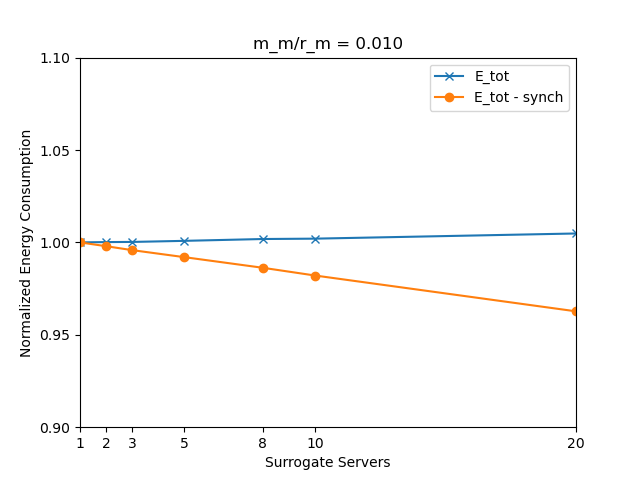
\includegraphics[width=8.1cm]{plots/sc40ratio0.01uniform.png}
	\end{center}
	\caption{$E_{tot}$ and $E_{tot - synch}$ for a Uniform cache policy, with a modify/request ratio of $0.01$ and a cache rate of $40\%$.}	
    \label{s2uniform0.01}
\end{figure}
\begin{figure}[!hbt]
	\begin{center}
		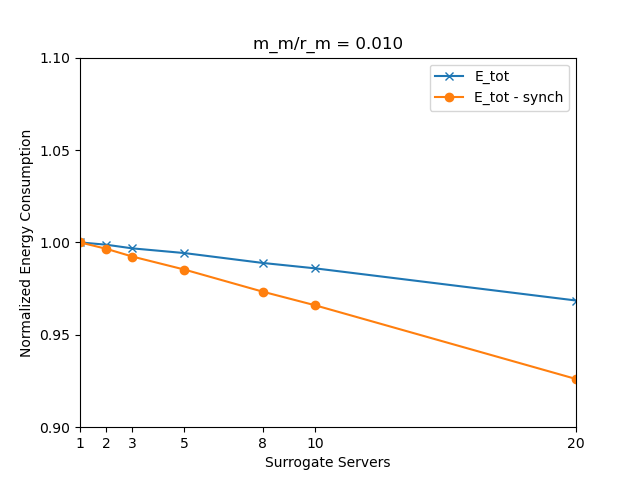
\includegraphics[width=8.1cm]{plots/sc40ratio0.01zipf.png}
	\end{center}
	\caption{$E_{tot}$ and $E_{tot - synch}$ for popularity-based cache policy, with a modify/request ratio of $0.01$ and a cache rate of $40\%$.}
    \label{s2zipf0.01}
\end{figure}


\section{3. Adaptations to Larger CDNs}
So far, the CDN energy consumption model we reference has been very useful for observing how to seek greener content delivery, alongside how using various cache policies affects energy usage. However, while working with the model, we also found some of the assumptions and constraints in \cite{biancoCDNs2017} to be unintuitive. In this section, we first examine the constraint on the amount of surrogates in our model, and then examine an important missing factor in our energy consumption calculations.

\subsection{3.1 Relaxing Surrogate Constraints}
Our above model makes the assumption that $S < T_2$ --- that there are fewer CDN surrogate servers than Tier 2 ISPs, and furthermore that there exists at most one surrogate per Tier 2 ISP. Reminding ourselves that in a realistic Internet hierarchy, Tier 2 ISPs are regional and national providers that operate both closer to clients than Tier 1 ISPs but further than Tier 3 ISPs, this assumption is unrealistic. If a large provider (e.g. TikTok or Spotify) wanted to rapidly deliver content, it would obviously want to have surrogates at as many Tier 3 ISPs as possible, regardless of whether they are connected to the same Tier 2 ISP. 

Furthermore, recalling our goal of optimizing CDN energy consumption, the results we found in previous sections seem to illustrate that adding surrogate servers consistently contributes to decreased normalized energy consumption. We realized this clearly couldn't be true, both in our model and in reality --- once there exists a surrogate in each Tier 3 ISP, there is no way to lower the amount of hops from a client to a surrogate. The only potential benefit of having several surrogates in a single Tier 3 ISP is redundancy, which we do not seek here because surrogates only contain part of the existing content, and our primary server is assumed to be stable. 

Given these two findings, we sought a way to update our constraint such that $S \leq T_3$ instead --- this follows from the fact that it could potentially be useful, and even energy-efficient, to continue adding surrogates until there is a surrogate at each Tier 3 ISP. As a result, we restructured our transmission energy consumption in order to allow for this new constraint. Namely, the probabilities $P_A, P_B, P_C$ of a client's closest hit being at a Tier 3, 2, or 1 ISP must be changed accordingly. 

For the purpose of interpretability, we shall assume that new surrogates will be uniformly randomly assigned to a Tier 3 ISP. Of course, this is not an entirely accurate assumption to make, since some Tier 3 ISPs have far higher priority than others, such as ones in more in-demand geographic areas (New York instead of Montana) or ones with a greater service population. However, our model already makes similar implicit assumptions, such as the fact that clients and surrogates are evenly geographically distributed. Furthermore, our model focuses on differentiating costs \textit{between} ISP tiers, and not \textit{within} them, so we shall leave this part to Future Work.

First, we calculate $P_A$ --- the probability that when a client requests a given piece of content, there exists a surrogate in the same Tier 3 ISP and it has that content. Here, we simply multiply the probability of a surrogate existing in that Tier 3 ISP ($\frac{S}{T_3}$ by uniformity) and the probability of a cache hit ($P_{hit}$, as calculated earlier). This gives us:
\[P_A = \frac{S}{T_3} \cdot P_{hit}\]
Next, we calculate $P_B$ --- the probability that the content could not be retrieved from a surrogate in the same Tier 3 ISP, but was able to be retrieved from a surrogate in the same Tier 2 ISP. First, we define a random variable for the amount of surrogates in a given Tier 2 ISP --- based on uniform selection without replacement, this gives us:
\[S_2 \sim \textrm{HGeom}(S, T_3-s, g_3)\]
Then, in order to formulate $P_B$, we summate over the amount of surrogates in a Tier 2 ISP where it is possible that a hit occurs --- this is 1 to $g_3$, since there cannot be a hit with 0 surrogates and there can also be at most 1 surrogate per Tier 3 ISP. Next, at each value in the summation, we calculate the probability of a hit for a Tier 2 ISP with that many surrogates --- this is $(1 - (1 - P_{hit})^i)$, since $(1 - P_{hit})^i$ defines the probability of none of the $i$ surrogates containing the requested content. Finally, we note that this summation includes scenario $A$, so we incorporate this to address overcounting:
\[P_B = \sum^{g_3}_{i=1}[P(S_2 = i) \cdot (1 - (1 - P_{hit})^i)] - P_A\]
\[P_B = \sum^{g_3}_{i=1}\left[\frac{\binom{S}{i}\binom{T_3-S}{g_3 - i}}{\binom{T_3}{g_3}} \cdot (1 - (1 - P_{hit})^i)\right] - P_A\]
Finally, $P_C$ accounts for the scenario that neither of the above occurred, and thus it is calculated as follows:
\[ P_C = 1 - (P_A + P_B)\]
Although this has ramifications on $E_{tx}$ as described above, our model otherwise remains unchanged. However, this opens up a new range of possible values for $S$, which is now constrained by $0 \leq S \leq T_3$ --- in 3.3, we shall see that this expanded range proves to be insightful.

\subsection{3.2 Incorporating Idle Energy Costs}
Another assumption made was that servers only incur an energy cost whenever actively processing a client's request. Although for larger CDNs this may effectively be true (since they are constantly performing computations),  we believe it is important to include an idle energy, even if it is minimal relative to the other forms of energy consumption in a CDN. This incorporates \cite{ulIslam2012}, which emphasizes the use of idle power as a potentially crucial aspect of CDN server utilization and energy consumption.

As a result, we shall accordingly make a slight modification to $E_{server}$, the total server costs of our CDN, in order to allow for a variable idle energy usage per surrogate server. We set $P_{idle}$ to a minimal value of $0.1W$ per server, taking the other model parameters into account while assuming high server utilization and optimization, but this can be changed for experimentation as needed. This allows us to formulate the following new formula:
\[E_{server} = S\cdot P_{idle}\cdot t + \sum_mBr_mP_{sr}\]
Analogously to section 4.1, we maintain the rest of the original model, and replace the old calculation for $E_{server}$ with the above formula.

\subsection{3.3 Results}
After incorporating the new modeling of $E_{tx}$ using $P_A, P_B, P_C$, and accounting for idle energy as described in 4.2, we can observe some new trends in our data that differ from what we find in 2.5. Firstly, we examine the values of $S$ as $\{2^0, 2^1, \ldots, 2^8 = 256\}$. In the graphs that do not include it, we still checked higher values of $S$ up to 1000 to verify end behavior, however the crossover point was found far sooner. 
\begin{figure}[!hbt]
	\begin{center}
		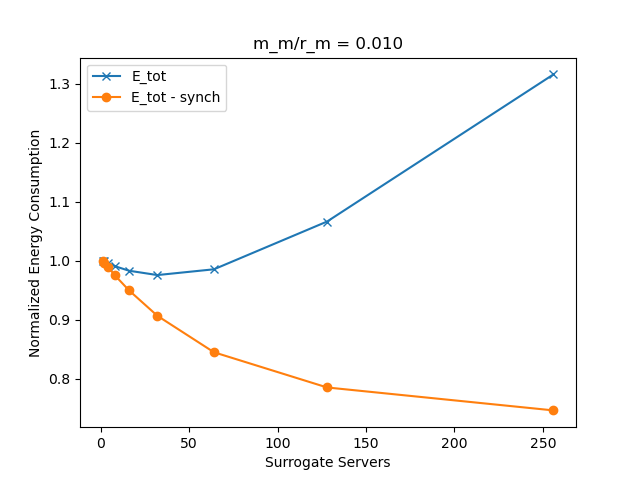
\includegraphics[width=8.1cm]{plots/new0.01.png}
	\end{center}
	\caption{Graphs of $E_{tot}$ and $E_{tot - synch}$ for a popularity-based cache policy, with a modify/request ratio of $0.01$ and a cache rate of $40\%$.}	
\label{new0.01}
\end{figure}
\begin{figure}[!hbt]
	\begin{center}
            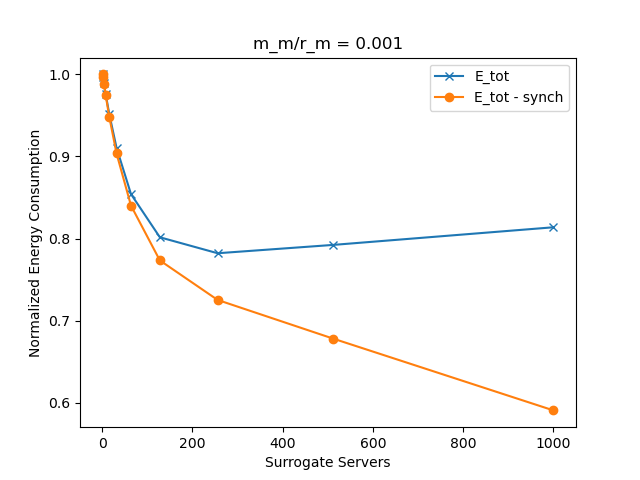
\includegraphics[width=8.1cm]{plots/new0.001.png}
	\end{center}
	\caption{Graphs of $E_{tot}$ and $E_{tot - synch}$ for a popularity-based cache policy, with a modify/request ratio of 0.001 and a cache rate of $40\%$.}	
\label{new0.001}
\end{figure}

As we can see in Figures ~\ref{new0.01} and ~\ref{new0.001}, the energy consumption of our CDN has very different behavior once extrapolated to a greater concentration of surrogate servers. Notably, we see that after a certain quantity of surrogate servers, the normalized energy consumption of our CDN reaches a minimum, forming an "elbow" after which it is no longer energy-efficient to add more surrogates. We see that this varies by the ratio of modified to requested content --- as this ratio increases, the crossover point decreases. This inverse proportionality makes sense: when much of the content being requested is also being modified, synchronization energy begins to dominate the overall CDN energy consumption, since this is a costly (and no longer rare) operation.

On the other hand, for CDNs with a very low $m_m/r_m$ ratio, it could prove beneficial to use a large amount of surrogate servers. For example, Spotify sees 100,000 song uploads per day while having users spend an hour a day listening to music --- with its 500 million listeners, this equates to approximately 10 billion songs per day \cite{spotifyUploads, headphonesaddict_2023}. Thus, Spotify has a $m_m/r_m$ ratio of $0.00001$, which means it would likely benefit from an even higher crossover point than represented in Figure ~\ref{new0.001}. This supports the reasoning behind our extension to the model in this section, in that modern, large-scale content providers like Spotify can benefit from having surrogate servers in all, or almost all, of the Tier 3 ISPs possible.

\section{4. A Better Cache Policy}

In addition to a limiting choice of model constraints, additional assumptions about the optimal cache policy as explained in \cite{biancoCDNs2017} do not necessarily hold. While \cite{biancoCDNs2017} asserts that Zipf with $\alpha = 0.8$ is an accurate caching policy for a variety of multimedia, content distributions on modern platforms like Tik Tok, Spotify, and YouTube all have different viewership patterns. This suggests that in some cases Zipf with $\alpha = 0.8$ may not be the best caching policy and alternate distributions could offer a better framework for CDN caching. 

Since platforms like Tik Tok and Spotify contain more items with high popularity that spontaneously change in popularity by going viral overnight, the distribution of popularity may be less skewed than Zipf with $\alpha = 0.8$ might suggest. Therefore, using the Zipf distribution to determine cache allocation especially for short-form video content may not be as effective as for other types of multimedia. Additionally, since short-form video content requires larger amounts of storage space, efficient cache allocation modeling is even more crucial to ensure optimal performance of a CDN. 

Instead of using Zipf with $\alpha = 0.8$, we build off of \cite{osmanthesis} and propose dynamically adjusting $\alpha$ based on different multimedia patterns. 

\subsection{4.1 Shortfalls of Zipf}

Popular platforms like Spotify and Tik Tok have an extremely high viewership rates. Spotify, for example, has $489$ million monthly active users \cite{headphonesaddict_2023}. Since the average Spotify user listens to approximately $720$ songs per month, we can estimate total monthly traffic as follows: 
\[
	489,000,000 \cdot 720 = 352.08 \texttt{ billion listens}
\]  
	
The most streamed Spotify song ever currently has $3.335$ billion streams. Averaged on a per-month basis since its release date in $2019$, we get $79,404,761$ monthly streams. Thus, on a given month, this song would be streamed with probability: 
\[
	\frac{79,404,761}{352,080,000,000} \approx 0.0023.
\] 

However, the Zipf distribution suggested by \cite{biancoCDNs2017} underestimates this probability. Recall that the frequency of viewership with a Zipf distribution for $i$ content objects ranked $i = 1, 2, \ldots, N$ is

\[
	P_N(i) = \frac{\Omega}{i^{\alpha}}
\] 

where 

\[
	\Omega = \left(\sum_{1}^{N} \frac{1}{i^{\alpha}}\right)^{-1}
\] 

by \cite{749260}. Since \cite{biancoCDNs2017} asserts that we should use parameter $\alpha = 0.8$, we fix $\alpha = 0.8$ for all our calculations with Zipf. 

Since there are approximately $80$ million songs on Spotify, Zipf would indicate that the probability of a stream on a given month being the most streamed song should be 

\[
	P_{80,000,000}(1) = \frac{\left(\sum_{1}^{80,000,000} \frac{1}{1^{0.8}}
	\right)^{-1}}{1^{0.8}} \approx 0.0000000125 \
\] 

which is an underestimate by a very large margin compared to our original calculation of $0.0023$.

Clearly, in the case of Spotify, the assertion that using Zipf with $\alpha = 0.8$ accurately captures content popularity patterns does not hold. These probability errors continue to compound for $i = 2, 3, 4, 5, \ldots, N$ because distances between the most popular types of content aren't consistent with what Zipf with $\alpha = 0.8$ would indicate. 

As \cite{osmanthesis} suggests, different popularity distributions of cached content exist in different video services. In order to optimize power and delay of video delivery, the ideal content to store in caches should be determined using the popularity distribution instead of relying solely on arbitrarily-distributed popularities according to Zipf ($\alpha$ = 0.8) as suggested by \cite{biancoCDNs2017}. 

For example, Real TV viewing data indicates that when the diversity of video popularities is high, storing the few most popular videos in caches minimizes power consumption, with power savings of up to 72\%. However, when video popularities are similar, the best power efficiency is achieved by maintaining variable caches in the network. In the context of the Zipf distribution, similarly popular video similarities might mean increasing the value of $\alpha$ to ensure the first ranked item isn't assigned an extremely high probability of a hit.

\subsection{4.2 Pareto Distribution}

In this section, we attempt to use a Pareto distribution with varying alpha values to demonstrate the impact on $P_{hit}$ calculations. For example, with an $\alpha = 1.16$ parameter, the Pareto principle (also known as the $80/20$ rule) would dictate that that 20\% of the content is responsible for 80\% of the views. This might be appropriate for certain types of content, such as movie streaming after a set of popular movie releases, which is why holding $\alpha = 0.8$ does not make sense. 

The Pareto distribution is essentially a continuous version of the Zipf distribution. The probability mass function (PMF) of the Pareto distribution can be mathematically expressed as:

\[
    P(X \geq x) = \left(\frac{x_m}{x}\right)^\alpha
\]

where $X$ is a random variable representing the size of a file, $x$ is the threshold size for caching, $x_m$ is the minimum file size for caching, and $\alpha$ is a parameter that controls the skewness of the distribution. Like the Zipf distribution, the Pareto distribution is a power law distribution, meaning that the ratio of frequencies of any two elements in the distribution is independent of the elements' actual values.  

\begin{figure}[h]
	\begin{center}
		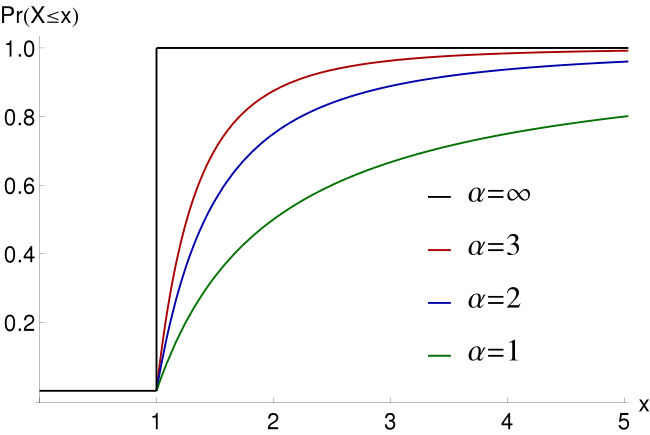
\includegraphics[width=8.1cm]{pareto.png}
	\end{center}
	\caption{A graph of the Pareto distribution CDF for various $\alpha$ with a scale parameter of $1$.}	
\end{figure}

The graph of the cumulative distribution function (CDF) of the Pareto distribution very strongly mirrors the Zipf distribution because both distributions are monotonically decreasing and positively skewed. 

\subsection{4.3 Pareto Energy Consumption}
Similar to section 2.3, we can calculate the cache hit probability for content that is distributed according to the Pareto distribution via the Pareto CDF. Since Pareto is continuous rather than discrete, we must however normalize our calculation to exclude assignments that exceed our document count. As such, the hit probability is as follows (note that the Pareto parameter $x_m=1$ is fixed):
\[ P_{hit}(\alpha, S_C, M) = \frac{1-\left(\frac{1}{MS_c}\right)^\alpha}{1-\left(\frac{1}{M}\right)^\alpha} \]
\noindent which we can then use to graph
\[ E_{tot}\left( P_{hit}(\alpha, 0.4, 1000), \ldots \right)\]
\noindent as a function of $\alpha > 0$, keeping all else constant:

\begin{figure}[h]
	\begin{center}
		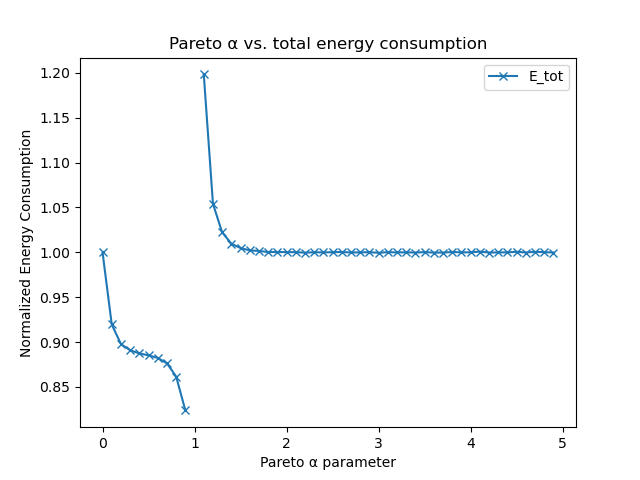
\includegraphics[width=8.1cm]{plots/pareto.png}
	\end{center}
	\caption{A graph of $E_{tot}$ for various $\alpha >0$ with $x_m = 1$.}	
        \label{paretoalpha}
\end{figure}

We note that the results from Figure~\ref{paretoalpha} follow intuitively as well. Once the Pareto $\alpha$ parameter surpasses one, $P_{hit}$ is effectively one. Hence increasing $\alpha$ further yields highly marginal improvements. The spiky behavior of the graph is accounted for by our random Poisson sampling for requests and modifications, and the marginal normalized energy consumption delta between $\alpha \approx 0$ and $\alpha =5$ is accounted for by the fact that $S$ was already fixed at the optimal \textit{crossover point}, as discussed in the prior section.

\section{5. Conclusions}

Our paper proposes a new model for the energy-efficient use of CDNs that takes into account a more realistic representation of network topology and improved cache policies. Our contributions are threefold:  a revised energy model that accounts for idle server energy consumption and permits for a larger amount of surrogates, a strategy with accompanying code to determine the optimal number of surrogate servers for a CDN with specific characteristics, and a more in-depth analysis of cache policies and their relationship to various types of online content.

Previous models are limited by their rigid network topology and the assumption that a Zipf distribution with parameter $\alpha=0.8$ accurately represents the popularity distribution of online content. By graphing the Pareto distribution with variable alpha, we were able to see that this parameter should be adjusted according to content type to accurately reflect the popularity distribution of online content. Additionally, the relaxation of surrogate constraints and the inclusion of idle energy costs improves previous energy consumption models, especially since previous models assume that adding surrogate servers linearly reduces energy consumption, which is inaccurate for a large amount of servers.

Despite the widespread use of CDNs, there remains little research on how to optimize them for energy consumption. CDNs play a vital role in the delivery of web content, and their use has only increased as more and more users come online. Optimizing CDNs to minimize energy consumption can have a significant impact on reducing the carbon footprint of the Internet. Through the creation of this paper, we hope to inspire further research in this important area to help create a more sustainable future for the internet. 

\section{6. Future Work}

\begin{figure}[h]
	\begin{center}
		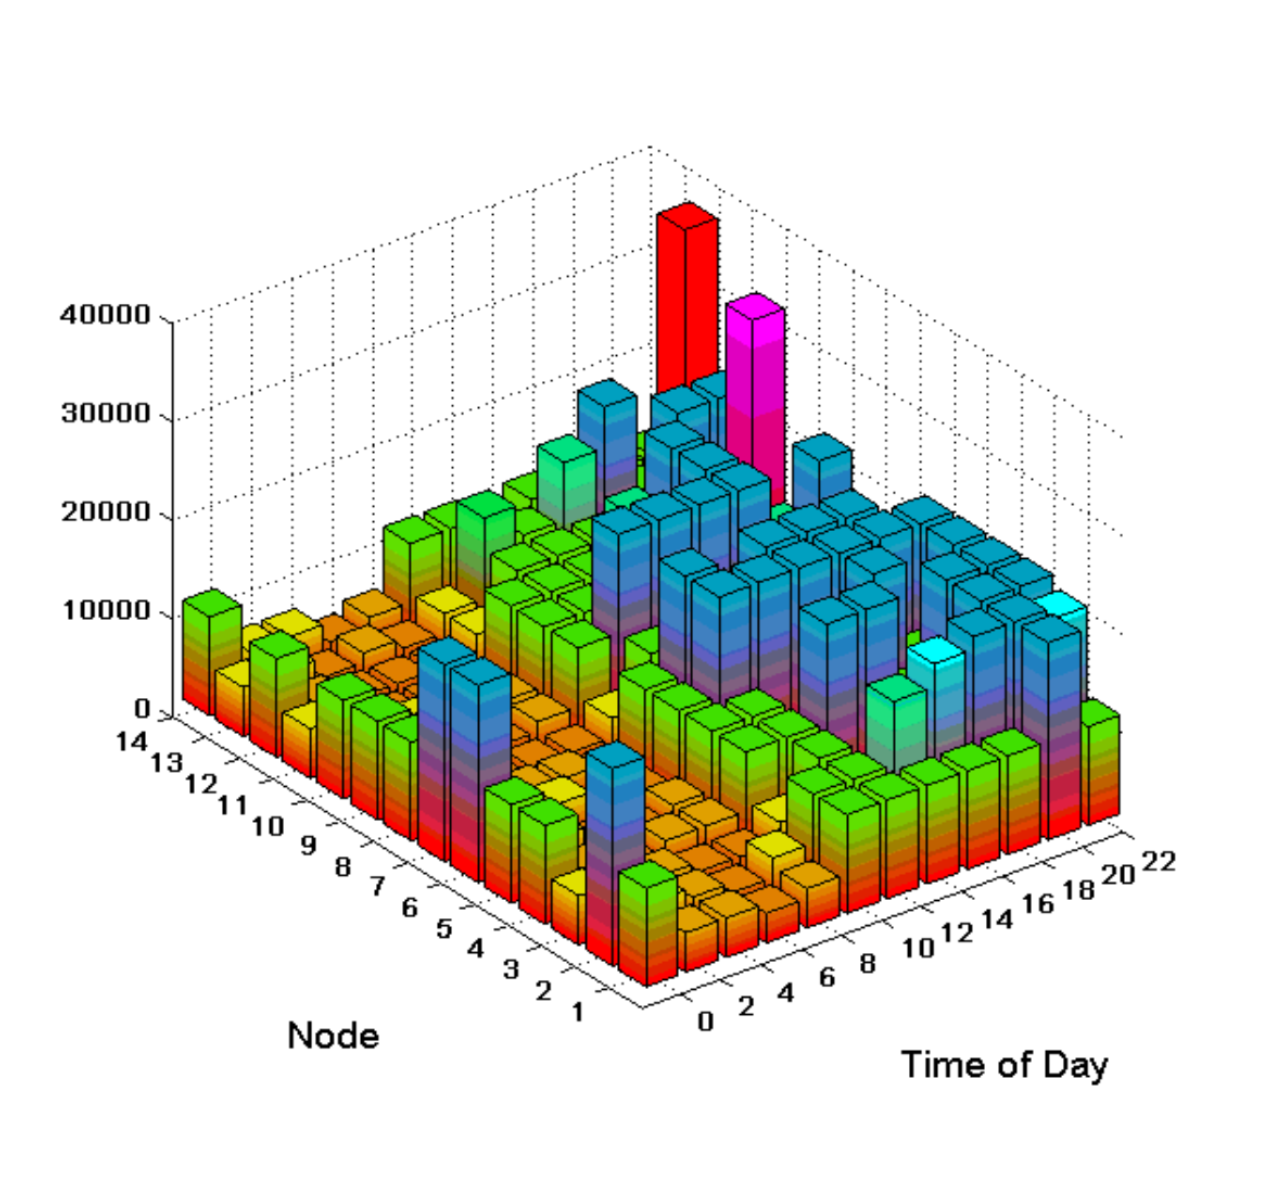
\includegraphics[width=8.1cm]{milp.png}
	\end{center}
	\caption{Optimal variable cache sizes for CDNs across nodes for different times of day, as computed by a MILP model.}	
\end{figure}


Although we have made significant improvements to existing models of energy consumption in CDNs, we recognize that our final model still provides a lack of clear strategic instruction, while also making numerous assumptions. These steps are intentional -- it is impossible to form a general analysis of CDNs, since they are widely used for services of varying size, data access patterns, and energy usage. As a result, we hope to have provided a more flexible model that can be used to guide initial paths to CDN energy conservation, based on generally-accepted cache policies and conservative model parameters.

One future area of work that could be synthesized productively with what we have presented is multi-integer linear programming (MILP). MILP can be used to optimize the allocation of content and server resources by creating a linear programming model that simultaneously maximizes cache hit rates, minimizes energy consumption, and optimizes the allocation of server resources. This method could provide a more precise and accurate analysis of CDN energy consumption by taking into account more factors than our proposed model. However, MILP models are computationally expensive and require a large amount of data to achieve the best results.


\printbibliography

\end{document}
